\documentclass[11pt,a4paper]{article}
\usepackage[margin=20mm]{geometry}
\usepackage{amsmath,amssymb,graphicx,booktabs,array}
\usepackage[colorlinks=true,urlcolor=blue,linkcolor=blue]{hyperref}
\usepackage[font=small,labelfont=bf]{caption}
\usepackage{microtype}
\setlength{\parindent}{0pt}
\setlength{\parskip}{6pt}
\graphicspath{{figures/}}
\hypersetup{pdftitle={Understanding the fourth-order interpolation benchmark}}
\newcommand{\pageheading}[1]{\clearpage\section{#1}}
\begin{document}
\begin{center}
{\Large\bfseries Understanding the fourth-order\\interpolation benchmark}\\[6pt]
{An explanation for an undergraduate physics student}\\[3pt]
{\small Production implementation: \texttt{e98eafcc}; figures: \texttt{de449678}}
\end{center}

\section{The question and the notation}
Imagine calculating vibrational properties of a crystal using only a small
periodic simulation cell. This gives information at a limited set of wavevectors.
Can we reconstruct the anharmonic interactions between those wavevectors and
obtain the same response as a calculation that knew the interactions on a much
denser mesh? That is the question tested here. It is especially demanding when
\emph{two phonons interact with two other phonons} through a fourth-order force constant.

The answer from this benchmark is yes, when the coarse mesh resolves the
interaction range. The fourth-order interpolation passed. A separate switch,
\texttt{ignore\_v3}, was incorrect and has been fixed. We will explain both statements.

Only the basic SSCHA/TD-SCHA notation below is used. Linear combinations of
displacements, variances, Fourier weights, and normalized vertices are written
out rather than assigned extra shorthand letters.

\begin{tabular}{@{}p{.22\linewidth}p{.74\linewidth}@{}}
\toprule
Notation & Meaning throughout this explanation \\
\midrule
$V$, $\mathcal R$, $u$ & Actual potential energy, mean atomic positions (centroids), and displacements from those means. Coordinates are mass weighted; $u_\ell$ is the molecular internal coordinate in cell $\ell$.\\
$\Phi$, $\omega_q$ & Auxiliary SSCHA harmonic force-constant matrix and its positive mode frequencies.\\
$\langle\cdots\rangle_{\rm SSCHA}$ & Average in the prescribed Gaussian SSCHA state.\\
$\Phi^{(3)},\Phi^{(4)}$ & Gaussian averages of the third and fourth derivatives of the actual potential, in mass-weighted coordinates.\\
$q,k,Q$ & Wavevectors; $Q$ is the externally excited wavevector, whereas $q,k$ run over internal phonon pairs. In this chain, wavevectors are in units of the reciprocal lattice period.\\
$N,N_c,N_f$ & Number of cells, equivalently wavevectors, on a periodic mesh; subscripts specify coarse and fine meshes. Integers $\ell,r,j$ and their primed versions are summation indices.\\
$T$, $n_{\rm B}(\omega_q)$ & Temperature and Bose occupation: $n_{\rm B}(\omega_q)=[\exp(\omega_q/(k_BT))-1]^{-1}$.\\
$G$, $\Pi$, $\Lambda$ & One-phonon Green function, dynamical self-energy, and harmonic two-phonon propagator. The short report calls the self-energy $\Sigma$; here we use $\Pi$ consistently.\\
$\omega$, $\eta$ & Applied frequency and positive numerical broadening; response functions are evaluated at $\omega+i\eta$.\\
$e_{a\alpha\nu}(q)$ & Phonon polarization: atom $a$, Cartesian component $\alpha$, mode $\nu$. Mode labels are suppressed for the single interacting branch.\\
\bottomrule
\end{tabular}

We set $\hbar$, the internal-coordinate mass, and the lattice spacing to one.
An asterisk denotes complex conjugation; a dagger denotes conjugate transpose.
Matrix inverses and sums retain their usual meanings. No abbreviations such as
$h$, $s$, $C$, $v$, $W$, or a named interpolation kernel are needed below.

\pageheading{A physical chain with a known harmonic reference}
Each cell contains a molecule with an internal vibration: the two atoms move
relative to one another. Its mass-weighted displacement is $u_\ell$. Translating
the entire crystal does not change this internal coordinate. Consequently an
energy depending on $u_\ell$ does not artificially pin the whole crystal.
Independent center-of-mass vibrations can be included as harmonic acoustic
branches. They do not enter the anharmonic potential in this benchmark.

The prescribed quadratic reference term is
\begin{equation}
 V_{\rm harmonic}=\frac12\sum_\ell u_\ell^2
                       +0.4\sum_\ell u_\ell u_{\ell+1}.
\end{equation}
The full potential below also contains quadratic counterterms. Thus this
reference matrix is not the bare Hessian of the full potential at zero
displacement; it will equal the \emph{Gaussian-averaged} Hessian.
The second term favours opposite internal distortions in neighbouring cells.
This is allowed for molecular internal coordinates; it is not the energy of a
single unstretched acoustic spring. The diagonal entries of $\Phi$ are one,
and the two nearest-neighbour off-diagonal entries are $0.4$.

Periodic boundary conditions mean that a displacement with a cell index beyond
the last cell is identified with its periodic image. The Fourier convention is
\begin{equation}
 u(q)=\frac1{\sqrt N}\sum_{\ell=0}^{N-1}u_\ell e^{-2\pi iq\ell},
 \qquad
 u_\ell=\frac1{\sqrt N}\sum_q u(q)e^{2\pi iq\ell}.
\end{equation}
On an $N$-point mesh, $q=0,1/N,\ldots,(N-1)/N$. Negative wavevectors are
understood modulo one. Real displacements obey $u(-q)=u(q)^*$.

Substituting this transform into the harmonic energy gives
\begin{equation}
 \omega_q^2=1+0.4e^{2\pi iq}+0.4e^{-2\pi iq}
           =1+0.8\cos(2\pi q).
\end{equation}
Every squared frequency lies between $0.2$ and $1.8$, so this harmonic reference
is stable. Its optical frequency is largest at the zone centre and smallest
at the zone boundary. An optical branch need not have its minimum at $q=0$.

This dispersion makes the decay test meaningful. A phonon at $Q=0$ can create
a pair at $q$ and $-q$, conserving momentum. Energy conservation requires
\begin{equation}
 \sqrt{1.8}=2\sqrt{1+0.8\cos(2\pi q)},
 \qquad \cos(2\pi q)=-0.6875.
\end{equation}
There are wavevectors satisfying this equation in the continuous Brillouin
zone. The phonon therefore lies inside a two-phonon continuum, not below every
possible decay channel. On a finite mesh, the allowed pair energies are discrete;
$\eta$ smooths those discrete features for comparison.

\textbf{What the harmonic reference means.} SSCHA uses an auxiliary harmonic
system to describe a Gaussian distribution of displacements. It does not
claim that the actual potential is harmonic. The auxiliary frequencies determine
how widely the atoms fluctuate, while derivatives of the actual potential
determine how those fluctuations interact.

\pageheading{The complete polynomial potential and its cutoff}
The actual potential adds three terms to the harmonic energy. Written without
abbreviating any displacement combination or variance, it is
\begin{align}
 V={}&\frac12\sum_\ell u_\ell^2+0.4\sum_\ell u_\ell u_{\ell+1}\notag\\
 &+\frac{0.08}{6}\sum_\ell\Big[
 (u_\ell+0.35u_{\ell+1})^3\notag\\[-2pt]
 &\hspace{25mm}-3\langle(u_\ell+0.35u_{\ell+1})^2\rangle_{\rm SSCHA}
                   (u_\ell+0.35u_{\ell+1})\Big]\notag\\
 &+\frac{0.12}{24}\sum_\ell\Big[
 (u_\ell+0.37u_{\ell+1}-0.29u_{\ell+2}+0.21u_{\ell+3})^4\notag\\
 &\quad-6\langle(u_\ell+0.37u_{\ell+1}-0.29u_{\ell+2}+0.21u_{\ell+3})^2
                   \rangle_{\rm SSCHA}\notag\\[-2pt]
 &\hspace{25mm}\times(u_\ell+0.37u_{\ell+1}-0.29u_{\ell+2}+0.21u_{\ell+3})^2\notag\\
 &\quad+3\langle(u_\ell+0.37u_{\ell+1}-0.29u_{\ell+2}+0.21u_{\ell+3})^2
                   \rangle_{\rm SSCHA}^{\,2}\Big]\notag\\
 &+\frac{0.04}{24}\sum_\ell\Big[
 (u_\ell-0.23u_{\ell+1})^4
 -6\langle(u_\ell-0.23u_{\ell+1})^2\rangle_{\rm SSCHA}
          (u_\ell-0.23u_{\ell+1})^2\notag\\
 &\hspace{25mm}+3\langle(u_\ell-0.23u_{\ell+1})^2\rangle_{\rm SSCHA}^{\,2}\Big].
\end{align}
\textbf{Every average appearing in this equation is a fixed numerical coefficient.}
It is evaluated once for a chosen coarse Gaussian, before evaluating energies,
forces, or fine-mesh responses. It is not differentiated with respect to an
instantaneous displacement and is not recomputed during interpolation.

The denominators $6=3!$ and $24=4!$ are convenient because differentiating three
or four times cancels the corresponding factorial. The cubic term makes the
energy asymmetric under $u\mapsto-u$ and couples one-phonon and two-phonon
fluctuations. The fourth-order terms couple pair fluctuations to one another.

No term contains cells separated by more than three lattice spacings.
Increasing $N_f$ changes the resolution of the wavevector integral, not the
interaction graph. This is the intended fixed cutoff: a fixed set of interacting
cells, not a displacement-dependent neighbour list.

The first quartic is genuinely a four-cell interaction:
\begin{equation}
 \frac{\partial^4 V}
 {\partial u_\ell\partial u_{\ell+1}\partial u_{\ell+2}\partial u_{\ell+3}}
 =0.12(1)(0.37)(-0.29)(0.21)=-0.00270396.
\end{equation}
An onsite quartic would never exercise this spatial structure. Finally, the
positive quartic terms stabilize large displacements. In particular
$|1-0.23e^{2\pi iq}|\geq0.77$: the second quartic has no unconstrained internal
Fourier direction. It eventually dominates the cubic and quadratic terms,
so the polynomial is bounded below.

\pageheading{Why the SSCHA reference stays fixed}
SSCHA selects the centroids and auxiliary force constants by minimizing the
variational free energy of a Gaussian state. At a stationary reference, in
mass-weighted coordinates, the relevant conditions are
\begin{equation}
 \left\langle\frac{\partial V}{\partial u_\ell}\right\rangle_{\rm SSCHA}=0,
 \qquad
 \Phi_{\ell\ell'}=
 \left\langle\frac{\partial^2 V}{\partial u_\ell\partial u_{\ell'}}
 \right\rangle_{\rm SSCHA}.
\end{equation}
These equations explain the apparently unusual linear and quadratic terms in
the potential. They make the prescribed Gaussian stationary for this model.
They do not establish that it is the global variational minimum.

For example, differentiating the cubic term centred on cell $\ell$ once with
respect to $u_\ell$ gives
\begin{equation}
 \frac{0.08}{2}\Big[(u_\ell+0.35u_{\ell+1})^2
       -\langle(u_\ell+0.35u_{\ell+1})^2\rangle_{\rm SSCHA}\Big].
\end{equation}
Its Gaussian average is exactly zero. A second derivative is proportional to
$u_\ell+0.35u_{\ell+1}$, whose average is also zero. Other derivative indices
only multiply these expressions by the appropriate numerical coefficients.

For the four-cell quartic, the second derivative of the term centred on $\ell$
with respect to $u_\ell$ is
\begin{align}
 \frac{0.12}{2}\Big[&(u_\ell+0.37u_{\ell+1}-0.29u_{\ell+2}+0.21u_{\ell+3})^2\notag\\
 &-\langle(u_\ell+0.37u_{\ell+1}-0.29u_{\ell+2}+0.21u_{\ell+3})^2
                 \rangle_{\rm SSCHA}\Big].
\end{align}
Again the average vanishes. Its first derivative has only odd powers, whose
averages vanish in a centred Gaussian. The last quartic works in exactly the
same way. Thus the anharmonic terms change neither the mean force nor the
mean curvature at the chosen reference.

The necessary variances are fixed by the harmonic frequencies:
\begin{align}
 \langle u_\ell u_{\ell'}\rangle_{\rm SSCHA}
 &=\frac1{N_c}\sum_{j=0}^{N_c-1}
 \frac{1+2n_{\rm B}(\omega_{j/N_c})}{2\omega_{j/N_c}}
              e^{2\pi i(j/N_c)(\ell-\ell')},\\
 \langle(u_\ell+0.35u_{\ell+1})^2\rangle_{\rm SSCHA}
 &=\frac1{N_c}\sum_{j=0}^{N_c-1}
 \frac{1+2n_{\rm B}(\omega_{j/N_c})}{2\omega_{j/N_c}}
              |1+0.35e^{2\pi i j/N_c}|^2.
\end{align}
The other two variances use the explicit four-cell and two-cell Fourier
polynomials given on the next page. At zero temperature the Bose occupations
vanish, but the variance remains nonzero: these are quantum zero-point fluctuations.

\textbf{An essential qualification.} A separately sampled fine periodic Gaussian
generally has a different covariance. The same potential need not be stationary
for both finite meshes. We therefore keep the chosen reference fixed and obtain
the fine anharmonic vertices analytically, rather than minimizing again or
silently changing the counterterms. Within each coarse-to-fine comparison the
potential is identical; different coarse meshes or temperatures define separate
controlled fixtures. This removes SSCHA minimization changes from the question
being tested.

\pageheading{Direct analytic vertices on any mesh}
The basic anharmonic quantities are Gaussian-averaged derivatives:
\begin{equation}
 \Phi^{(3)}_{\ell_1\ell_2\ell_3}
 =\left\langle\frac{\partial^3 V}
 {\partial u_{\ell_1}\partial u_{\ell_2}\partial u_{\ell_3}}
 \right\rangle_{\rm SSCHA},\qquad
 \Phi^{(4)}_{\ell_1\ell_2\ell_3\ell_4}
 =\left\langle\frac{\partial^4 V}
 {\partial u_{\ell_1}\partial u_{\ell_2}\partial u_{\ell_3}\partial u_{\ell_4}}
 \right\rangle_{\rm SSCHA}.
\end{equation}
The cubic polynomial has constant third derivatives. The quartic polynomial
contributes a linear displacement to the third derivative, whose centred
Gaussian average vanishes. Fourth derivatives of a quartic are constants.
The counterterms have degree at most two and cannot change either vertex.
Therefore these vertices are known exactly, without sampling, and do not depend
on the Gaussian covariance when its mean remains zero.

To see where the wavevector dependence comes from, Fourier-transform one
linear combination explicitly:
\begin{equation}
 u_\ell+0.35u_{\ell+1}
 =\frac1{\sqrt N}\sum_q
       (1+0.35e^{2\pi iq})u(q)e^{2\pi iq\ell}.
\end{equation}
Cubing this expression gives three Fourier factors. Summing over cells enforces
$q_1+q_2+q_3=0$ modulo a reciprocal lattice period. The resulting intensive
vertices, with the momentum-conserving constraint understood, are
\begin{align}
 \Phi^{(3)}(q_1,q_2,q_3)
 &=0.08\prod_{j=1}^{3}(1+0.35e^{2\pi iq_j}),\\
 \Phi^{(4)}(q_1,q_2,q_3,q_4)
 &=0.12\prod_{j=1}^{4}
   (1+0.37e^{2\pi iq_j}-0.29e^{4\pi iq_j}+0.21e^{6\pi iq_j})\notag\\
 &\quad+0.04\prod_{j=1}^{4}(1-0.23e^{2\pi iq_j}).
\end{align}
These are explicit finite trigonometric polynomials, not fitted functions.
Evaluating them at every fine wavevector produces the \emph{direct analytic
fine reference}. It uses no coarse data and no interpolation routine.
For example, at $Q=0$ the cubic vertex reduces to
\begin{equation}
 \Phi^{(3)}(-q,q,0)=0.12123+0.0756\cos(2\pi q).
\end{equation}
Its value at any intermediate $q$ can be evaluated immediately, without a fit.

\textbf{Why the mesh factors appear.} Each displacement Fourier transform
contributes $N^{-1/2}$, while the sum over the common cell contributes $N$.
The actual coupling between normalized modes is therefore
\begin{equation}
 \frac{\Phi^{(3)}(q_1,q_2,q_3)}{\sqrt N},
 \qquad
 \frac{\Phi^{(4)}(q_1,q_2,q_3,q_4)}{N}.
\end{equation}
Going from coarse to fine normalized mode couplings requires
$\sqrt{N_c/N_f}$ for third order and $N_c/N_f$ for fourth order. These are not
adjustable corrections and must not be applied twice. The intensive vertices
in the preceding equations themselves have no such mesh dependence.

At fixed external momentum $Q$, a pair is $(q,Q-q)$. Cubic coupling connects
that pair to the single mode at $Q$, through
$\Phi^{(3)}(-q,q-Q,Q)$. Quartic coupling connects it to a second pair
$(k,Q-k)$, through $\Phi^{(4)}(-q,q-Q,k,Q-k)$. There are therefore
\emph{two independent internal momenta} in the fourth-order problem.

\pageheading{Analytic Fourier interpolation without new shorthand}
Now suppose the potential is not available analytically at arbitrary momenta,
but its vertices are known at the nine coarse points $j/9$. To reconstruct the
value at $q$, multiply each coarse sample by
\begin{equation}
 \frac19\sum_{r=-4}^{4}e^{2\pi i(q-j/9)r}.
\end{equation}
This expression is written out each time below. It is a Fourier interpolation
weight, not a linear interpolation between two neighbouring samples.
It follows from a discrete inverse Fourier transform: the coefficient of
harmonic $r$ in the cubic pair vertex is
\begin{equation}
 \frac19\sum_{j=0}^{8}
 \Phi^{(3)}(-j/9,j/9-Q,Q)e^{-2\pi i(j/9)r}.
\end{equation}
Multiplying this by $e^{2\pi iqr}$, summing over $r=-4,\ldots,4$,
and interchanging the two sums gives the weight above.
At $q=j'/9$ it is one if $j=j'$ and zero otherwise. This follows from the sum
of equally spaced complex phases around the unit circle.

For the intensive cubic vertex the interpolation is
\begin{align}
 &\Phi^{(3)}_{\rm interpolated}(-q,q-Q,Q)\notag\\
 &\quad=\sum_{j=0}^{8}
 \left[\frac19\sum_{r=-4}^{4}e^{2\pi i(q-j/9)r}\right]
 \Phi^{(3)}(-j/9,j/9-Q,Q).
\end{align}
For the quartic vertex both internal momenta must be reconstructed:
\begin{align}
 &\Phi^{(4)}_{\rm interpolated}(-q,q-Q,k,Q-k)\notag\\
 &=\sum_{j=0}^{8}\sum_{j'=0}^{8}
 \left[\frac19\sum_{r=-4}^{4}e^{2\pi i(q-j/9)r}\right]
 \Phi^{(4)}(-j/9,j/9-Q,j'/9,Q-j'/9)\notag\\
 &\hspace{35mm}\times
 \left[\frac19\sum_{r'=-4}^{4}e^{-2\pi i(k-j'/9)r'}\right].
\end{align}
The opposite signs on the two Fourier factors express conjugate-transpose
reconstruction on the incoming and outgoing pair spaces. For this simple
odd scalar mesh the weights happen to be real. In the atom-resolved production
problem they need not be real, so the conjugation is essential.

\textbf{Why this is exact for the benchmark.} At fixed $Q$, the exponent of the
$q$ dependence is the difference of two cell positions belonging to one
interaction. The same is true independently for $k$. Each difference lies
between $-3$ and $3$ for the unrebased scalar model. Nine samples distinguish
all Fourier harmonics from $-4$ to $4$, so no relevant harmonic is lost or
confused with another. Seven odd-grid samples would suffice for the unrebased
scalar support; the main benchmark deliberately uses nine.

Three samples cannot do this. On the three-point mesh,
$e^{2\pi i(j/3)3}=1$: an interaction at separation three looks identical to one
at separation zero. This is \emph{aliasing}. The coarse information no longer
specifies the correct off-grid vertex, even if every coarse sample is exact.

This explains the two analytic calculations used as controls: directly evaluate
the explicit polynomial at fine momenta, or evaluate it only at coarse momenta
and apply the Fourier sums above. Their agreement is a mathematical check.
\textbf{It is not by itself a test of the production code.} The next step
replaces the analytic coarse contraction with the actual force-based Julia
contraction, while retaining the direct analytic fine result as the reference.

\pageheading{What the production interpolation actually computes}
Constructing every fine-mesh fourth-order tensor entry would be expensive.
TD-SCHA instead needs the \emph{action} of this tensor on a pair perturbation.
The double interpolation sum can be evaluated in the opposite order: first
sum the incoming fine perturbation into coarse pair space, act there, then
reconstruct the outgoing fine pair. This is ordinary reassociation of finite
sums, not a new physical approximation.

\begin{enumerate}
\item The code starts with a fine-mesh pair perturbation. It applies the
frequency/occupation factors of the TD-SCHA representation and transforms
mode components into mass-weighted Cartesian components.
\item It sums the perturbation onto coarse momenta using the conjugate of the
explicit Fourier weight on the previous page. This is the \emph{fold}.
\item It applies the inverse Gaussian covariance factors on the coarse mesh.
For the interacting branch, the inverse variance of a mode is explicitly
\begin{equation}
 \frac{1}{\langle u(q)u(-q)\rangle_{\rm SSCHA}}
       =\frac{2\omega_q}{1+2n_{\rm B}(\omega_q)}.
\end{equation}
These factors must be evaluated on the same coarse reference as the sampled
forces. Using the fine frequencies here would change the estimated vertex.
\item The actual Julia routine contracts the coarse displacements and
anharmonic force residuals. It applies the factors $\sqrt{N_c/N_f}$ and
$N_c/N_f$ for the cubic and quartic contributions.
\item The result is reconstructed on the fine mesh using the adjoint Fourier
operation, transformed back into fine phonon modes, and given the final
TD-SCHA frequency factors. The harmonic part uses the prescribed fine
frequencies throughout.
\end{enumerate}

For example, the coarse force residual includes the following derivative
of the complete cubic energy:
\begin{align}
 -\frac{\partial V_{\rm cubic}}{\partial u_\ell}
 =-\frac{0.08}{2}\Big[&(u_\ell+0.35u_{\ell+1})^2
        -\langle(u_\ell+0.35u_{\ell+1})^2\rangle_{\rm SSCHA}\notag\\
 &+0.35\big((u_{\ell-1}+0.35u_\ell)^2
        -\langle(u_{\ell-1}+0.35u_\ell)^2\rangle_{\rm SSCHA}\big)\Big].
\end{align}
The quartic residual is cubic in the displacements. The production test
provides these polynomial forces, not an analytic fourth-order tensor in
place of the Julia contraction.

\textbf{Atoms, phases, and pair counting.} For several atoms the code uses
$u_{a\alpha}(q)=\sum_\nu e_{a\alpha\nu}(q)u_\nu(q)$ on each pair leg. It centres
the real-space images according to atom positions and the actual cell metric;
only equally near images share a boundary weight. Thus the simple scalar
Fourier sum is a teaching version of the atom-resolved operation, not a
replacement for it. Reassigning an atom to a neighbouring cell changes Fourier
phases but cannot change the physical result.

Finally, $(q,Q-q)$ and $(Q-q,q)$ are the same physical pair. The direct
reference sums over both ordered orientations. Production stores unique
pairs and supplies the corresponding multiplicities; equal-momentum pair
blocks are complex symmetric and use a transpose, not a conjugate transpose,
for exchanging the two legs. Testing phases and these factors is essential.

\pageheading{From vertices to the bubble and the full response}
The harmonic two-phonon propagator is diagonal in the ordered pair index.
With $q$ and $k$ on the fine mesh, its diagonal entry is
\begin{align}
 \Lambda_{qq}(Q,\omega+i\eta)
 =-\frac{1}{4\omega_q\omega_{Q-q}}\Bigg[
 &\frac{(\omega_q+\omega_{Q-q})
 [1+n_{\rm B}(\omega_q)+n_{\rm B}(\omega_{Q-q})]}
 {(\omega_q+\omega_{Q-q})^2-(\omega+i\eta)^2}\notag\\
 -&\frac{(\omega_q-\omega_{Q-q})
 [n_{\rm B}(\omega_q)-n_{\rm B}(\omega_{Q-q})]}
 {(\omega_q-\omega_{Q-q})^2-(\omega+i\eta)^2}\Bigg].
\end{align}
Off-diagonal entries are zero. The first denominator describes creating or
annihilating a phonon pair. The second describes converting a thermally
occupied phonon into another phonon. At zero temperature its numerator is
zero. This expression includes the pair-counting convention used by the
ordered-pair reference; changing to unique pairs requires matching factors.

Without the fourth-order interaction the self-energy is the bubble:
\begin{equation}
 \Pi_{\rm bubble}(Q,\omega+i\eta)
 =\frac1{N_f}\sum_q
 |\Phi^{(3)}(-q,q-Q,Q)|^2\Lambda_{qq}(Q,\omega+i\eta).
\end{equation}
A single phonon becomes a pair through one cubic vertex, propagates as a
harmonic pair, and returns through the other cubic vertex.

With fourth order included, the pair can interact repeatedly before returning.
In pair-space matrix notation the full expression is
\begin{align}
 \Pi(Q,\omega+i\eta)=\frac1{N_f}\sum_{q,k}
 &\Phi^{(3)}(-q,q-Q,Q)^*\notag\\[-3pt]
 &\times\left[\Lambda(Q,\omega+i\eta)^{-1}
                -\frac{\Phi^{(4)}}{N_f}\right]^{-1}_{qk}
 \Phi^{(3)}(-k,k-Q,Q).
\end{align}
Here the $qk$ entry of the fourth-order matrix is explicitly
$\Phi^{(4)}(-q,q-Q,k,Q-k)$. The outer inverse is a \emph{matrix inverse over
pair momenta}, not a reciprocal taken separately for each entry. An equivalent
form without an inverse of $\Lambda$ is
$[I-\Lambda\Phi^{(4)}/N_f]^{-1}\Lambda$, where $I$ is the ordinary identity matrix.
The matrix inverse includes arbitrarily many repeated quartic interactions;
it is not just one additional perturbative diagram. It remains a TD-SCHA
response, not the exact many-body response of the anharmonic Hamiltonian.

The one-phonon Green function is
\begin{equation}
 G(Q,\omega+i\eta)
 =\frac{1}{(\omega+i\eta)^2-\omega_Q^2-\Pi(Q,\omega+i\eta)}.
\end{equation}
The real self-energy shifts resonances. Its imaginary part describes coupling
to pair excitations. For a narrow, weakly frequency-dependent resonance, the
spectral half-width is approximately
$-\operatorname{Im}\Pi(Q,\omega_Q+i0^+)/(2\omega_Q)$. The reciprocal of this
half-width is the amplitude-decay time; the population-decay time differs by
a factor of two. Strongly frequency-dependent or overlapping peaks require
the full response rather than this approximation. Numerical $\eta$ is a
regulator, not automatically a physical inverse lifetime.

\pageheading{How the comparison excludes misleading agreements}
\textbf{Exact averaging, actual production contractions.}
Random Monte Carlo samples would leave statistical errors in the vertices.
Here the Gaussian averages are evaluated with deterministic quadrature.
The polynomial force has degree at most three, and the Julia estimator
multiplies it by at most three displacement factors. Its total degree is
therefore at most six. The quadrature is exact through degree seven, with
only floating-point roundoff remaining. Some quadrature weights are negative;
they are integration coefficients, not probabilities for a stochastic ensemble.

Independent harmonic coordinates have vanishing connected anharmonic
contributions and are integrated out analytically. Only the interacting
internal-coordinate Gaussian requires quadrature. The fixture supplies the
prescribed harmonic modes and ensemble arrays directly; it exercises the
real production fold, Julia contraction, reconstruction, and full operator.
It is not an end-to-end SSCHA minimization or ensemble-file-loading test.

\textbf{Three different comparisons.}
\begin{enumerate}
\item Evaluate the explicit analytic vertices at every fine wavevector,
then calculate the fine response. This is the independent reference.
\item Use only coarse forces and Gaussian displacements in production,
interpolate the operator to the fine mesh, then calculate the response with
the same fine harmonic frequencies, temperature, and broadening.
This must agree with the first calculation when the support is resolved.
\item Calculate responses at several coarse \emph{external} wavevectors,
then interpolate the response itself to an intermediate external wavevector.
This is generally a different answer, even when every input response uses
the same fine internal momentum sum.
\end{enumerate}

The last distinction is important. Fourier reconstruction of a finite-range
vertex is exact once all its harmonics are known. The Green function contains
an inverse of a frequency-dependent matrix. Inversion does not preserve the
finite range. Even the harmonic expression
\begin{equation}
 \frac{1}{(\omega+i\eta)^2-1-0.8\cos(2\pi Q)}
\end{equation}
is not a finite trigonometric polynomial in $Q$. It can contain arbitrarily
long Fourier harmonics, despite the nearest-neighbour harmonic potential.
Thus ``interpolate the vertices, then respond'' need not equal ``respond,
then interpolate.'' The latter is a control, not the acceptance criterion.

Production refines \emph{internal} pair momenta at an external $Q$ already
on the coarse mesh. The off-grid external-$Q$ comparison in the report is
analytic: it does not demonstrate a capability the production class lacks.
Its approximately $31\%$ discrepancy at $Q=1/18$ measures response
interpolation over the chosen frequency window, not a production failure.

\textbf{What agreement does and does not establish.} At fixed $N_f$ and $\eta$
we test whether interpolation implements the same TD-SCHA operator as the
analytic potential. This isolates interpolation from minimization, sampling,
and iterative-solver truncation. A physical lifetime still requires increasing
$N_f$ at fixed $\eta$, then reducing $\eta$ while refining the mesh further.
Matching two finite-mesh curves is not, by itself, that convergence study.

\pageheading{Reading the response figures}
\begin{figure}[ht]
\centering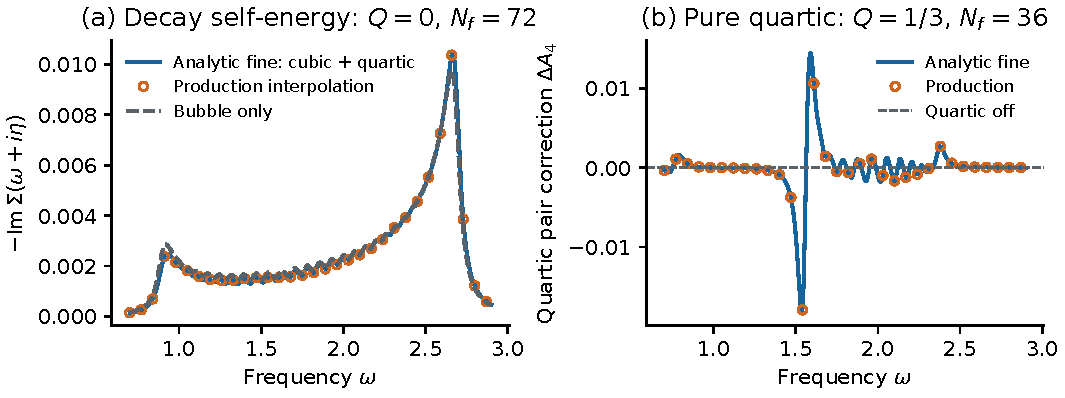
\includegraphics[width=\linewidth]{response.pdf}
\caption{The production simulations from the concise report. The internal
coarse mesh has nine points and the numerical broadening is $\eta=0.04$.
Panel (a) has $Q=0$, $N_f=72$, and $T=0$. Panel (b) has $Q=1/3$,
$N_f=36$, and $k_BT=0.3$. The plotted data and generating script accompany
this explanation. The figure uses $\Sigma$ for the self-energy denoted by
$\Pi$ in the text.}
\end{figure}

\textbf{Left panel: coupling of a phonon to the pair continuum.}
The blue curve is the imaginary self-energy computed from the analytic
fine-mesh vertices, including repeated quartic pair interactions. Orange
circles come from the production calculation starting with coarse forces.
The circles lie on the blue curve. The dashed curve has fourth order
switched off, so it is the bubble alone.

The difference between the dashed and solid curves is the measurable
beyond-bubble contribution. In this plotted frequency window the relative
norm of the complex full-minus-bubble self-energy is approximately $6.9\%$.
The relative norm of the production-minus-analytic full self-energy is about
$1.6\times10^{-13}$. These are two different comparisons: a sizeable physical
quartic contribution and a tiny numerical interpolation error.

The peak near the upper end of the two-phonon band is not automatically the
linewidth of the externally excited phonon. This graph shows the self-energy
as a function of applied frequency; the external harmonic mode is at
$\omega_0=\sqrt{1.8}$. The one-phonon response and its resonance also depend
on the real self-energy through the denominator of $G$.

\textbf{Right panel: isolate fourth order completely.}
Both cubic couplings are disabled, so a one-phonon probe cannot reach pair
space. Instead, the graph examines the pair-space response directly. It
subtracts the pair response with fourth order disabled from the pair response
with fourth order included. The vertical quantity labelled $\Delta A_4$ in
the original figure means precisely this difference of normalized spectral
traces; it is a diagnostic of pair dynamics, not a Raman intensity without
specifying a Raman perturbation.

The normalization divides the trace by the number of pair coordinates in
the tested TD-SCHA representation. The same representation is used on both
sides. Blue and orange again coincide, while the dashed zero line represents
no quartic interaction. A positive or negative correction is allowed: the
interaction redistributes spectral weight. The relative error in the
\emph{unsubtracted} pair spectral trace is about $1.6\times10^{-15}$.

This second panel is particularly valuable. Agreement in a one-phonon
spectrum alone could hide an inaccurate small quartic correction under a
large harmonic or cubic contribution. Directly isolating pair dynamics
removes that ambiguity.

\pageheading{Accuracy, deliberate failures, and the actual fix}
\begin{figure}[ht]
\centering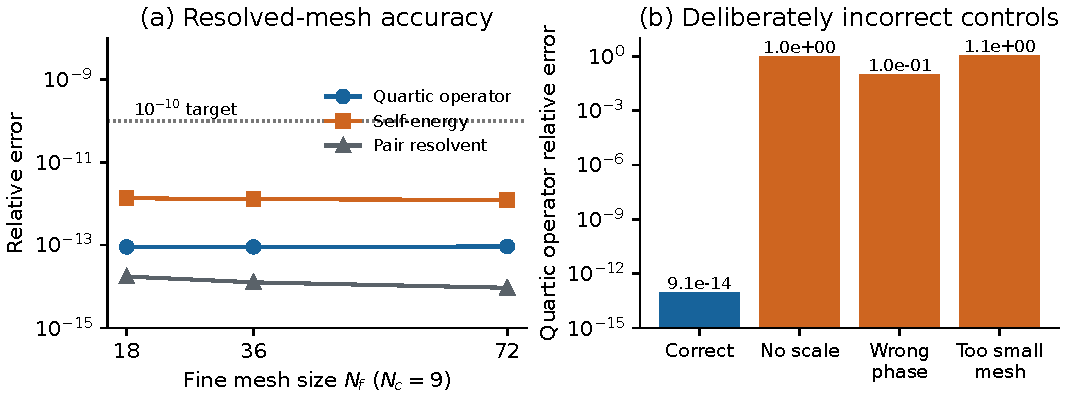
\includegraphics[width=\linewidth]{accuracy.pdf}
\caption{Numerical accuracy and sensitivity controls. Left: $N_c=9$,
$Q=1/3$, $k_BT=0.3$, with $N_f=18,36,72$. Right: zero-temperature controls;
the first three bars use $9\to18$, $Q=1/3$, and the last $3\to18$, $Q=0$.
``Wrong phase'' means an incorrectly conjugated interpolation kernel.}
\end{figure}

The quartic error is the Euclidean norm of all entries of the production-minus-
analytic quartic operator, divided by the corresponding analytic norm. The
harmonic block is subtracted first, so it cannot hide quartic errors. The
self-energy and pair-resolvent errors are the largest relative errors over
41 frequencies between $0.3$ and $2.8$, with $\eta=0.04$.

The quartic error stays near $9\times10^{-14}$ as the fine mesh grows. The
self-energy error stays near $10^{-12}$. These are interpolation errors at
each mesh, not errors relative to the infinite-crystal limit. Their small,
flat values show that changing the coarse-to-fine normalization does not
introduce a systematic error. The dashed $10^{-10}$ line is the operator/
resolvent tolerance; the self-energy acceptance tolerance is $10^{-8}$.

The deliberately wrong cases are informative. Removing $N_c/N_f$ causes an
order-one quartic error. Incorrect conjugation causes roughly $10\%$ error.
A three-point coarse mesh aliases the fixed three-cell interaction and also
fails by order one. A test unable to detect these changes would provide much
weaker evidence. The full regression suite also checks even meshes, unequal
masses, atom rebasing, complex mixing of mode vectors, acoustic masks, and
independent cubic/quartic switches: 56 tests passed, including 16 new tests.

\textbf{Was the code right or wrong?} The fourth-order interpolation itself was
right in these resolved-support tests. The bug concerned the switch
\texttt{ignore\_v3}: it suppressed the one-phonon-to-pair cubic coupling but
left the pair-to-one-phonon coupling active. These two couplings should be
adjoints under the TD-SCHA pair metric. Removing only one spoils that relation
and prevents a clean pure-quartic test. Both directions are now disabled in
both q-space classes. Calculations with cubic coupling enabled are unchanged
by this particular fix. The tests establish the stated finite-range benchmark;
they are not a guarantee for unresolved interactions or every possible model.

\small
\textbf{Reproduction and background.} The implementation, numerical data, and
plotting script are in \path{benchmarks/interpolation/}; see its
\texttt{README.md} for the test command. The equations above are derived for
that explicit polynomial and its code conventions. For broader theory, see
\href{https://arxiv.org/abs/2103.03973}{Monacelli et al., the SSCHA review (2021)}
and \href{https://arxiv.org/abs/2011.14986}{Monacelli and Mauri, TD-SCHA (2021)}.
\end{document}
